\section{One inventory problem, different predictive states}
The economic problem is the same across this study: quote on both sides, collect execution revenue, and control the risk and cost of carrying inventory. What changes is the state required to predict continuation risk. We organize the models into Markovian diffusion benchmarks, non-Markovian memory drivers and finite Markovian approximations of those drivers. The comparisons then separate policy behavior from numerical accuracy.

With cash $X$, inventories $q$ and mid-prices $S$, terminal wealth is $X_T+q_T^\top S_T-L(q_T,Y_T)$, where $L=0$ for the historical diffusion benchmark and a declared close-out penalty applies in the liquidation experiments. Unit fills update cash and inventory together; arrival intensities are $Ae^{-k\delta}$. CARA utility has risk aversion $\gamma>0$~\cite{AvellanedaStoikov2008}. Shared notation does not imply identical parameter settings or a common absolute PnL scale.

\section{Markovian price models and portfolio risk}
For ABM, $dS=\sigma\,dW$; for GBM, $dS=\mu S\,dt+\sigma S\,dW$. Their current price is a Markov state. The ABM finite-horizon inventory penalty is $\frac\gamma2q^2\sigma^2(T-t)$ and the reservation level is $S-q\gamma\sigma^2(T-t)$. Under the classical exponential-arrival approximation, the total quoted spread is
\[
\gamma\sigma^2(T-t)+\frac{2}{\gamma}\log(1+\gamma/k).
\]
The GBM reservation rule uses the local monetary variance $(\sigma S)^2$; the Gaussian ABM derivation is not an exact GBM--CARA solution. In a correlated diffusion, the corresponding risk penalty is $\frac\gamma2(T-t)q^\top\Sigma q$, with inventory pressure $\Sigma q$. A second asset's position therefore changes a quote even without volatility memory.

This benchmark establishes the intersection with the memory models: the relevant quantity is future inventory covariance, not inventory size alone. Constant covariance makes the risk forecast tractable. A history-dependent variance state changes that forecast, while a finite factor approximation changes how it is computed. The extended derivations and original diffusion figures are retained in the unified companion~\cite{hft1}.

\section{Non-Markovian memory and finite Markovian lifts}
A causal Gaussian driver can be represented as $Y_t=\int_0^t K(t-s)\,dB_s$. A general memory kernel retains information from past shocks. Fractional Brownian motion with $H\ne0.5$ is a non-Markovian reference~\cite{MandelbrotVanNess1968}; a generic current scalar value is insufficient to close its dynamics. The kernel $K\equiv1$ instead gives a Brownian causal check. A fractional-like Volterra kernel need not produce standard fBM covariance.

Approximating $K$ by $\sum_m w_me^{-\lambda_m t}$ gives
\[
dZ_m=-\lambda_mZ_m\,dt+dB,\qquad Y=\sum_mw_mZ_m.
\]
The full finite vector $Z$ is Markovian. Its aggregate generally is not a closed scalar Markov state because
\[
dY=-\sum_mw_m\lambda_mZ_m\,dt+\Bigl(\sum_mw_m\Bigr)dB.
\]
Two vectors with the same $Y$ can have different aggregate drifts. Replacing this with a scalar OU surrogate is a second approximation, separate from approximating the original kernel~\cite{AbiJaberElEuch2019,hft2}. The positive Laplace-mixture identity for the singular rough kernel applies to $H<0.5$. Historical finite-factor cases labelled $H=0.5$ and $H=0.8$ are weight-rule configurations; the former is not exact Brownian motion and the latter is phenomenological, not that identity extended beyond its range.

In the two-asset experiment, each asset has six factors with logarithmic rates from 3 to 180 and normalized weights $w_m\propto\lambda_m^{-0.7}$. Prices remain conditionally diffusive, $dS_i=\sigma_i(Y_i)dW_i$, with
\[
\sigma_i^2(Y_i)=1.1^2\exp(0.75Y_i-0.5\,0.75^2v_Y).
\]
Price correlation is $\rho=0.7$, factor-driver correlation $\nu=0.35$, and price/factor noise is independent. The full twelve-factor environment is a \emph{finite Markovian approximation}, not a directly solved non-Markovian HJB. Covariance $\Sigma_{AB}=\rho\sigma_A\sigma_B$ is stochastic even though $\rho$ is fixed.

\section{Reduced controls and the complete equation}
The liquidation experiments use $A=14$, $k=1.15$, $\gamma=0.2$, $T=1$, inventory limits $|q_i|\le6$ and offsets in $[0.02,4]$. Terminal cost is
\[
L(q,Y)=\sum_i\{(0.60+0.28\sigma_i(Y_i))|q_i|+0.18q_i^2\}.
\]
With $U=-\exp[-\gamma(X+q^\top S+\theta)]$, $\theta(T,q,Z)=-L(q,Y)$. The scalar surrogate uses drift $-1.35Y$, variance coefficient $0.20955182706132114$ and stationary variance $v_Y=0.0776117878004893$. Matching that stationary variance does not match the aggregate's instantaneous diffusion or close its drift.

\subsection{Bounded numerical solution and full residual}
For a neighbor gain $g=\theta(q+e_i)-\theta(q)$, define the bounded arrival Hamiltonian
\[
 h(g)=\max_{\delta\in[0.02,4]}\frac{Ae^{-k\delta}}{\gamma}\{1-e^{-\gamma(\delta+g)}\},\qquad
 \delta^*(g)=\operatorname{clip}_{[0.02,4]}\!\left(\frac{\log(1+\gamma/k)}{\gamma}-g\right).
\]
An analogous neighbor difference gives the ask. Prohibited inventory transitions are absent from the operator. Clipping the controls is distinct from clipping the value surface. The historical HFT2 calculation clipped the value; the positive HFT3 baseline solves in $u=\exp(-\gamma\theta)$ with nonnegative state-transition rates and CFL-controlled explicit steps, checking positivity rather than projecting the value onto fixed limits.

For the twelve-dimensional factor covariance $Q$, rates $\lambda$, and inventories $q$, the complete residual is
\begin{align}
\mathcal H[\theta]={}&\theta_t-\sum_{im}\lambda_mZ_{im}\theta_{Z_{im}}+
 \tfrac12 Q:(D^2\theta-\gamma\nabla\theta\nabla\theta^\top)
 -\tfrac\gamma2 q^\top\Sigma q\\
 &+\sum_i\big[\mathbf1_{q_i<6}h(\theta(q+e_i)-\theta(q))+
 \mathbf1_{q_i>-6}h(\theta(q-e_i)-\theta(q))\big].
\end{align}
All mixed factor derivatives matter. A reduced scalar solve can have a small residual in its own declared generator while its immersion has a substantial complete residual. Therefore numerical error, boundary truncation, interpolation error and state-compression defect must be diagnosed separately.

The existing baseline exports 41 times over nine grid/domain configurations. The runtime interpolates $\theta$ linearly in physical time and the aggregate state, forms discrete inventory differences, then optimizes the bounded Hamiltonian. It counts state-domain clamps rather than silently assuming extrapolation is valid. Refactoring this lookup into a common module gives a maximum offset difference of $5.33\times10^{-15}$ across 5,000 comparisons with the historical implementation. This is numerical replay equivalence, not a speed measurement.

A proposed localized correction would use $\theta_{j+1}=\theta_j+\chi_j\sum_kc_k\Phi_k$, retain time, spatial and mixed product derivatives of the gate, and recompute the complete nonlinear residual on an evaluation set distinct from the fit set. A reduction criterion is an acceptance test, distinct from stopping on absolute tolerance, stagnation or budget. No such fitted correction is claimed in this paper.


\paragraph{C++ implementation.}
The same bounded Hamiltonian and derivative-aware operator are evaluated independently in C++. The current work exports a positive baseline and tests scalar embedding, mixed derivatives and gate products. It does not fit correction coefficients. Offline precomputation, policy interpolation and dense-factor simulation have distinct costs; no local operation count establishes exchange latency or an online speedup.

\section{Comparative results within each model class}
The results below answer different questions under declared experiments. We compare policies \emph{within} each setting and interpret their common inventory mechanism, without pooling mean PnL across different terminal costs, initial states and solvers.

\subsection{Diffusion benchmarks and memory-inspired scalar policies}
In the 5000-path ABM replay, inventory-sensitive quotes lower terminal marked-PnL mean from 67.145 to 63.930 and its standard deviation from 12.178 to 6.680; mean absolute terminal inventory falls from 7.817 to 3.116. The local-variance GBM replay has the same direction: mean PnL 67.109/63.894 and dispersion 12.316/6.718. The 3000-path correlated-diffusion comparison lowers portfolio-risk norm from 17.051 to 7.419 while mean marked PnL falls from 158.709 to 154.556. These results concern Markovian prices without rough memory.

The historical six-factor forward simulations instead use forced liquidation and a clipped scalar HJB policy. In 2000 sessions at the weight-rule label $H=0.2$, mean liquidated PnL is 4.955/3.309 for naive/HJB, while mean pre-close absolute inventory is 2.504/0.547 and sample CE 2.052/2.352. The labels $H=0.5$ and $H=0.8$ also show lower mean PnL and higher reported CE for the historical inventory-aware policy. These are results of the clipped implementation, not proof of convergence or of an optimal policy for the original memory process.

With a positive bounded baseline, the 300-path E1/E2 replay asks whether that policy controls inventory in its scalar and lifted environments. E2 mean liquidated PnL is 4.792/7.607 for naive/P2, with paired difference 2.816 (SE 0.240), and pre-close absolute inventory 2.613/0.427. E1 reports paired PnL difference 2.279 (SE 0.215). These within-environment gains do not isolate the causal effect of replacing the historical clipped solver: the experiment configuration also differs.

\subsection{Stochastic-covariance proxy and risk--revenue trade-off}

The separable policy evaluates $\theta_{sep}=\theta_0(t,q_A,Y_A)+\theta_0(t,q_B,Y_B)$. The explicit candidate
\[
 C_{cov}=-\gamma(T-t)\Sigma_{AB}(Y)q_Aq_B
\]
approximates the omitted cross-risk under covariance frozen at its current level over the remaining horizon. For asset B its raw bid offset shifts by $+\gamma(T-t)\Sigma_{AB}q_A$ and its ask by the negative of that amount, before bounds are applied. Asset A uses the inventory in B. This is a covariance proxy, not a residual-fitted P3 policy \cite{BergaultEvangelistaGueantVieira2022,multifactor}.

The quote shift is conditional, not an instruction to sell a real security. A unit sale in B changes portfolio variance by $-2(\Sigma q)_B+\Sigma_{BB}$, which is negative only in the appropriate inventory region. A sufficiently large hedge can make another unit sale increase risk. The correction vanishes at $T$, retaining the declared terminal cost.

The experiment uses 400 paired paths, seed 73, 3900 intervals, initial $S=(100,100)$, $q=(3,0)$ and $X=-300$: initial marked wealth is zero. Policy pairs share price and factor shocks, candidate arrival times, asset/side marks and acceptance uniforms. A total Poisson candidate rate of 56 is thinned with $\exp(-1.15\delta)$, and quotes/inventory update sequentially. Prices and volatility remain frozen during arrivals within a step, giving a disclosed splitting error.

OU transitions use exact Gaussian innovations on the time grid, with
\[
 Q^{\Delta t}_{im,jn}=\nu_{ij}\frac{1-e^{-(\lambda_m+\lambda_n)\Delta t}}{\lambda_m+\lambda_n}.
\]
Spectral factorization removes only roundoff-negative eigenvalues under a relative guard. The representative path is path zero fixed before inspecting outcomes. The second step size is a diagnostic; it is not coupled-path convergence evidence.

\begin{table}[ht]\centering\small
\caption{Synthetic paired experiment, 400 paths and 3900 steps.}
\begin{tabular}{lrr}\toprule
Metric & Separate P2 & Covariance proxy\\\midrule
Integrated variance, mean & 5.844280 & 4.960778\\
Liquidated PnL, mean & 14.433479 & 14.090451\\
Sample CARA certainty equivalent & 12.305356 & 12.234514\\
Absolute A inventory before close & 0.5275 & 0.5300\\
Absolute B inventory before close & 0.4825 & 0.5200\\\bottomrule
\end{tabular}\end{table}
The paired risk difference is $-0.883503$ (SE $0.108498$); the paired PnL difference is $-0.343028$ (SE $0.090778$). Integrated risk falls about 15.1\%, while mean PnL and sample utility do not improve. Integrated inventory variance is not the empirical variance of terminal PnL. A 10,000-resample paired bootstrap gives a sample certainty-equivalent difference of $-0.070843$, with percentile 95\% interval
\[
[-0.398632,\ 0.288272].
\]
The interval includes zero, so the negative sample difference is not evidence of a population utility loss. This concerns sampling conditional on this model, not parameter uncertainty.

\begin{figure}[p]\centering
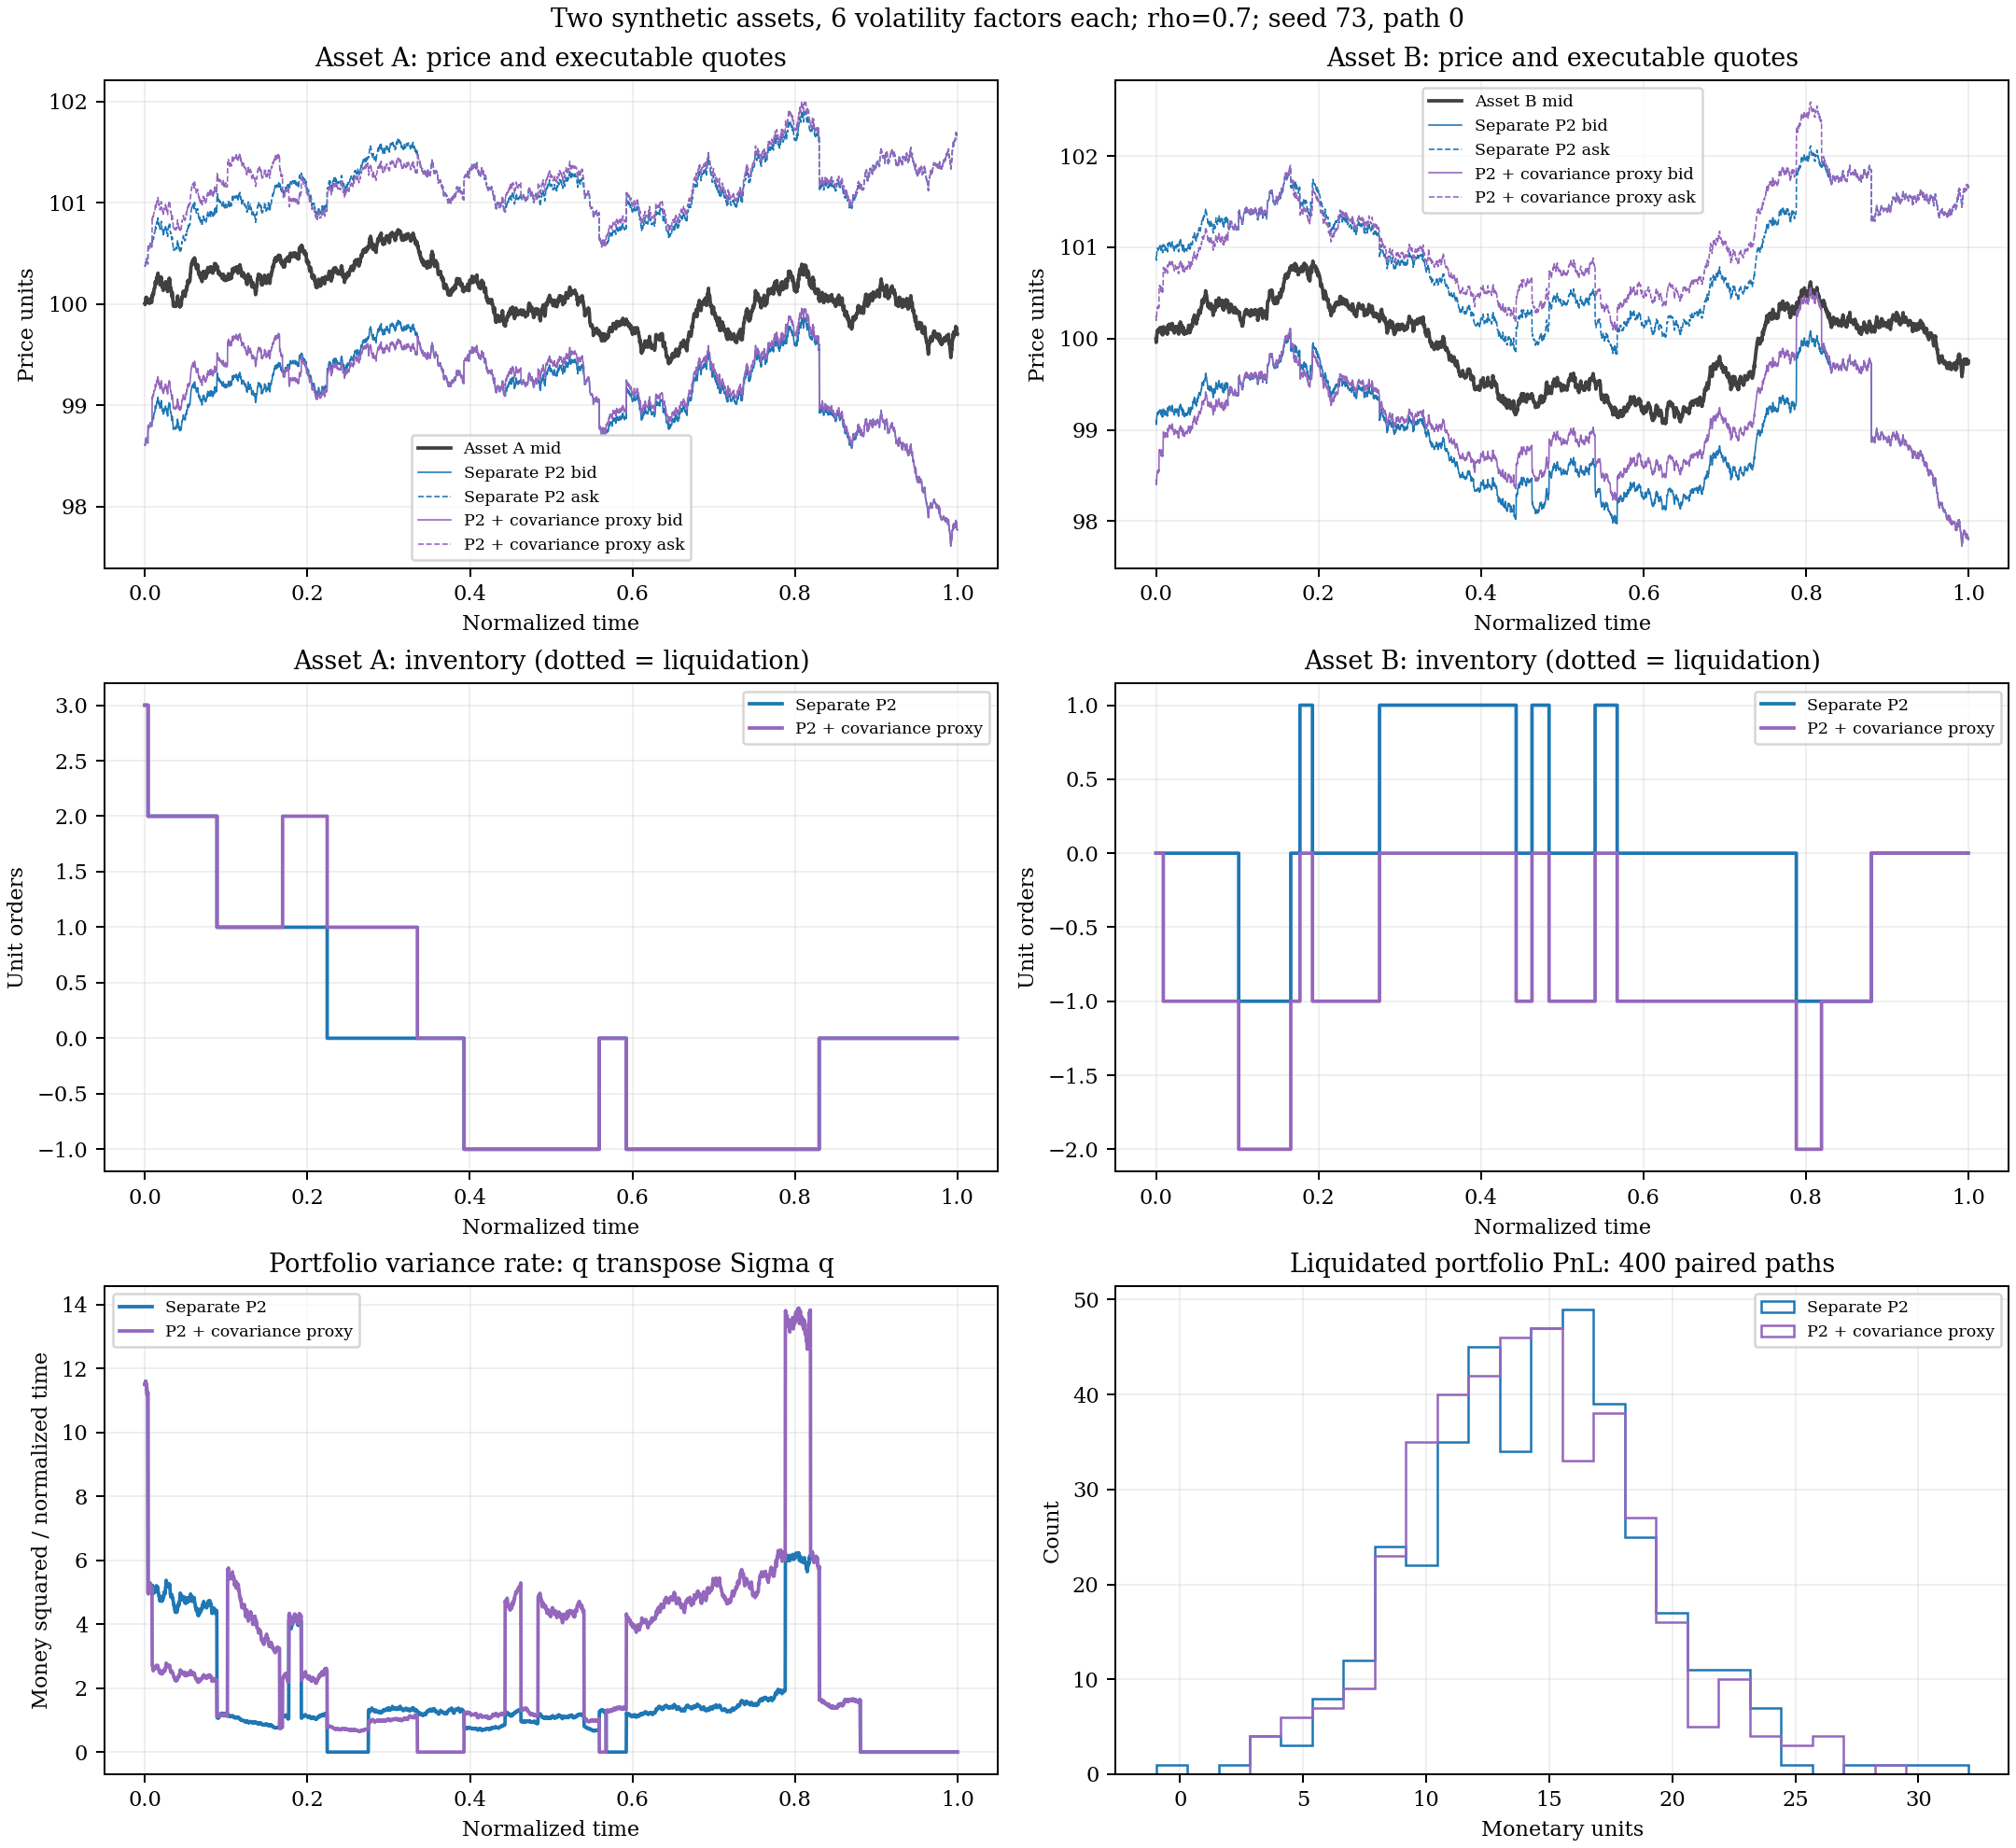
\includegraphics[width=\textwidth]{img/hft3-multiasset_inventory.png}
\caption{Two synthetic assets under the paired policies: quotes, inventory and portfolio variance along fixed path zero; terminal PnL histogram over all paths. Lower instantaneous risk on a displayed segment is not proof of higher utility.}
\end{figure}

\subsection{Residual diagnostics and numerical sensitivity}

Economic replay and operator checks address separate acceptance criteria. At $\rho=0$, separate and proxy quotes, inventory and cash coincide in the regression test; this does not prove exact HJB separability with correlated volatility drivers. Accounting checks keep maximum floating-point discrepancies below $1.6\times10^{-13}$ and the reported main runs contain no out-of-domain policy lookup. Recompiled C++ suites pass the 528 operator/correction checks, positive-baseline tests and multi-asset operator tests. Independently evaluating the 3000 exported separate/proxy jets in C++ agrees with Python to maximum absolute discrepancy $1.67\times10^{-13}$. Test success establishes the checked implementation identities, not optimality.

The new off-grid full-operator diagnostic uses 1500 stationary factor samples, seed 20261013, inventories from $-6$ to $6$ and times in $[0.05,0.95]$. There are 1379 samples with both aggregates inside two stationary standard deviations. Baseline derivatives are reconstructed by cubic splines. Covariance derivatives are analytic: $\nabla C=Ca$, $D^2C=Caa^\top$, $a_{im}=0.75w_m/2$, and $\partial_t C=\gamma\Sigma_{AB}q_Aq_B$. Nonlinear arrivals and the factor-correlation gradient term are recomputed after adding the correction.

\begin{table}[ht]\centering
\caption{Interior off-grid residual RMS; derivative-reconstruction diagnostic.}
\begin{tabular}{lr}\toprule
Operator/policy & RMS\\\midrule
Sum of reduced scalar residuals & 0.004638\\
Complete operator, separate baseline & 2.481440\\
Complete operator, covariance proxy & 5.069320\\\bottomrule
\end{tabular}\end{table}
The complete residual becomes larger under the proxy in this diagnostic. The frozen/no-arrival cross-risk cancellation identity cannot be used to infer improvement under stochastic covariance and arrivals. The derivative reconstruction has not been certified against an independently converged low-dimensional reference, so the RMS values are diagnostics rather than value-error bounds.

Additional solves isolate time refinement, fixed-spacing domain refinement and spatial refinement, with actual effective step counts recorded. The following differences use common interior points at $t=0,0.5$ and every inventory.
\begin{table}[ht]\centering\small
\caption{Finite-resolution differences against each family's finest configuration.}
\begin{tabular}{lrr}\toprule
Comparison & Max value diff. & Max offset diff.\\\midrule
9360 vs 18720 steps & 0.0009573 & 0.0002740\\
5SD vs 6SD, fixed spacing & 0.0000014 & 0.00000034\\
161 vs 241 state nodes & 0.0003235 & 0.0002459\\\bottomrule
\end{tabular}\end{table}
These are finite-resolution differences, not rigorous error estimates. Coupled simulation-step convergence, derivative convergence, a reduced full-HJB reference and fitted-policy preservation remain necessary before a stronger correction claim.

The model omits queue position, adverse selection and exchange latency, and uses synthetic uncalibrated inputs. No local software benchmark is interpreted as trading-venue latency. The exact Navier--Stokes source mentioned by the design brief remains unverified; the mathematical operator and diagnostics here stand on their own, and no theorem transfers from that proposed analogy. Exact correspondence of the received manuscripts to the historical reference PDFs remains a documentary limitation; the original versions are retained.


\section*{Conclusion}
The organizing distinction is the predictive state. Markovian diffusions give a tractable inventory-risk benchmark; non-Markovian drivers motivate richer volatility information; finite Markovian lifts permit recursive simulation; scalar compression makes the control problem small while changing its generator. All of these layers share cash--inventory accounting, but their performance evidence is conditional on different experiments.

Inventory control reduces exposure in the classical and historical finite-lift comparisons; the positive baseline also improves paired liquidated PnL in its own E1/E2 replay. A further covariance proxy lowers accumulated price risk but lowers sample PnL/CE and increases the reconstructed full residual. This reconciles the apparent conflict between favorable inventory statistics and an inadequate complete-equation correction. A fitted P3 requires independent reference and convergence gates plus economic checks; it is not supplied by the present hedge, software tests or proposed architectural analogy.
